\documentclass[12pt,a4paper]{article}
\usepackage[utf8]{inputenc}
\usepackage[slovak]{babel}
\usepackage[siunitx]{circuitikz}
\usepackage{listings}
\usetikzlibrary{arrows,chains,matrix,positioning,scopes,shapes.geometric}
\usepackage[T1]{fontenc}
\usepackage{natbib}
\usepackage{graphicx}
\usepackage{amsmath}
\usepackage{makeidx}
\usepackage{graphicx}
\usepackage{tikz}
\usepackage{physics}
\usepackage[left=2cm,right=2cm,top=2cm,bottom=2cm]{geometry}
\usepackage{hyperref}
\usepackage{title_page}
\usepackage{booktabs, multirow, tabularx}
\usepackage{booktabs}
\usepackage{gensymb}

\hypersetup{
    colorlinks=true,
    linkcolor=blue,
    filecolor=magenta,      
    urlcolor=cyan,
}

\definecolor{codegreen}{rgb}{0,0.6,0}
\definecolor{codegray}{rgb}{0.5,0.5,0.5}
\definecolor{codepurple}{rgb}{0.58,0,0.82}
\definecolor{backcolour}{rgb}{0.95,0.95,0.92}


\lstdefinestyle{mystyle}{
    backgroundcolor=\color{backcolour},   
    commentstyle=\color{codegreen},
    keywordstyle=\color{magenta},
    numberstyle=\tiny\color{codegray},
    stringstyle=\color{codepurple},
    basicstyle=\ttfamily\footnotesize,
    breakatwhitespace=false,         
    breaklines=true,                 
    captionpos=b,                    
    keepspaces=true,                 
    numbers=left,                    
    numbersep=5pt,                  
    showspaces=false,                
    showstringspaces=false,
    showtabs=false,                  
    tabsize=2
}
\lstset{style=mystyle}


\title{Semestrálny projekt \\ Základy elektrotechniky}
\author{Pavel Kratochvíl \hfill xkrato61}

\date{December 2020}

\begin{document}

    \maketitle
    \newpage
    \tableofcontents
    \section{Príklad č.~1} 

\subsection{Zadanie}
Stanovte napätie $U_{{R}_6}$ a prúd $I_{{R}_6}$ s použitím metódy zjednodušovania. \\

\begin{table}[ht]
	\centering
	\begin{tabular}{|c|c|c|c|c|c|c|c|c|c|c|}
		\hline
		sk. & $U_{1}$~[V] & $U_{2}$~[V] & $R_{1}~[\Omega]$ & $R_{2}~[\Omega]$ & $R_{3}~[\Omega]$ & $R_{4}~[\Omega]$ & $R_{5}~[\Omega]$ & $R_{6}~[\Omega]$ & $R_{7}~[\Omega]$ & $R_{8}~[\Omega]$ \\
		\hline
		A& 80& 120& 350& 650& 410& 130& 360&750 &310 &190  \\
		\hline
	\end{tabular}
\end{table}

\subsection{Zjednodušovanie obvodu}

\begin{figure}[h!]
\begin{circuitikz} \draw

(0,7) to[dcvsource, v_=$U_1$](0,3.5)
(0,3.5) to[dcvsource, v_=$U_2$](0,0)
(0,7) -- (1.5,7)
(1.5,7) to[R, l_=$R_1$](5,7)
(1.5,7) to[R, *-*, l=$R_2$](1.5,3.5)
(5,7) to[R, *-*, l_=$R_5$](5,3.5)
(1.5,3.5) -- (1.5,2)
(1.5,3.5) to[R, *-*, l_=$R_3$](5,3.5)
(1.5,2) to[R, *-*, l_=$R_4$](5,2)
(5,3.5) -- (5,2)
(5,7) -- (8.5,7)
(8.5,7) to[R, -*, l_=$R_7$, ](8.5,3.5)
(8.5,4.5) -- (8.5,3.5)
(5,3.5) to[R, *-*, l=$R_6$, i=$I_6$, v=$U_6$](8.5,3.5)
(0,0) to[R, l_=$R_8$](8.5,0)
(8.5,3.5) -- (8.5,0)
;

\end{circuitikz}
\centering
\caption{Pôvodný obvod}
\end{figure}
\clearpage

\begin{figure}[h!]
\begin{circuitikz} \draw
(0,7) to[dcvsource, v_=$U_1$](0,3.5)
(0,3.5) to[dcvsource, v_=$U_2$](0,0)
(0,7) -- (1.5,7)
(1.5,7) to[R, l_=$R_1$](5,7)
(1.5,7) to[R, *-*, l=$R_2$](1.5,3.5)
(5,7) to[R, *-*, l_=$R_5$](5,3.5)
(1.5,3.5) to[R, *-*, l_=$R_3{_4}$](5,3.5)
(5,7) -- (8.5,7)
(8.5,7) to[R, -*, l_=$R_7$, ](8.5,3.5)
(8.5,4.5) -- (8.5,3.5)
(5,3.5) to[R, *-*, l=$R_6$, i=$I_6$, v=$U_6$](8.5,3.5)
(0,0) to[R, l_=$R_8$](8.5,0)
(8.5,3.5) -- (8.5,0)
;
\end{circuitikz}
\centering
\caption{Spojenie $R_3$ a $R_4$}
\end{figure}

\begin{equation*}
\begin{aligned}
R_3{_4} &=\frac{R_3 R_4}{R_3+R_4} \\
\end{aligned}
\end{equation*}

\begin{figure}[h!]
\begin{circuitikz} \draw

(0,5.25) to[dcvsource, v_=$U_1$](0,2.75)
(0,2.75) to[dcvsource, v_=$U_2$](0,0)
(0,5.25) -- (1.5,5.25)
(1.5,7) to[R, l_=$R_1$](5,7)
(5,7) to[R, *-*, l_=$R_5$](5,3.5)
(1.5,7) -- (1.5,3.5)
(1.5,3.5) to[R, -, l_=$R_2{_3}{_4}$](5,3.5)
(8.5,7) -- (8.5,3.5)
(5,7) to[R, *-, l_=$R_7$, ](8.5,7)

(5,3.5) to[R, *-, l=$R_6$, i=$I_6$, v=$U_6$](8.5,3.5)
(0,0) to[R, l_=$R_8$](10,0)

(10,0) -- (10,5.25)
(8.5,5.25) -- (10,5.25)
;
\end{circuitikz}
\centering
\caption{Spojenie $R_2$ a $R_3{_4}$}
\end{figure}

\begin{equation*}
\begin{aligned}
R_2{_3}{_4} &= R_3{_4} + R_2 \\
\end{aligned}
\end{equation*}

\clearpage

\begin{figure}[h!]
\begin{circuitikz} \draw

(0,5.25) to[dcvsource, v_=$U_1$](0,2.75)
(0,2.75) to[dcvsource, v_=$U_2$](0,0)

(0,5.25) to[R, l=$R_A$](2.5,5.25)
(2.5,5.25) to[R, *-*, l=$R_B$](5,7)
(2.5,5.25) to[R, *-*, l_=$R_C$](5,3.5)

(8.5,7) -- (8.5,3.5)
(5,7) to[R, *-, l_=$R_7$, ](8.5,7)

(5,3.5) to[R, *-, l=$R_6$, i=$I_6$, v=$U_6$](8.5,3.5)
(0,0) to[R, l_=$R_8$](10,0)

(10,0) -- (10,5.25)
(8.5,5.25) -- (10,5.25)
;
\end{circuitikz}
\centering
\caption{Trojuholník -> hviezda}
\end{figure}


\textit{Vytvorenie rovníc na prevod trojuholník -> hviezda: \\}
\begin{equation*}
\begin{aligned}
R_A&=\frac{R_1R_{234}}{R_1+R_{234}+R_5} \\
R_B&=\frac{R_1R_5}{R_1+R_{234}+R_5} \\
R_C&=\frac{R_5R_{234}}{R_1+R_{234}+R_5} \\
\end{aligned}
\end{equation*}


\begin{equation*}
\begin{aligned}
R_B{_7} &=R_B+R_7 \\
R_C{_6} &=R_C+R_6 \\
R_B{_7}{_C}{_6} &=\frac{R_B{_7}R_C{_6}}{R_B{_7}+R_C{_6}} \\
\end{aligned}
\end{equation*}

\begin{figure}[h!]
\begin{circuitikz} \draw
(0,4) to[dcvsource, v_=$U_1$](0,2)
(0,2) to[dcvsource, v_=$U_2$](0,0)
(0,4) to[R, l=$R_A$](4.75,4)
(4.75,4) to[R, l=$R_B{_7}{_C}{_6}$](8.5,4)
(0,0) to[R, l_=$R_8$](10,0)
(10,0) -- (10,4)
(8.5,4) -- (10,4)
;
\end{circuitikz}
\centering
\caption{Sériové spojenie $R_B$ a $R_7$, $R_C$ a $R_6$; paralelné spojenie $R_B{_7}$ a $R_C{_6}$.}
\end{figure}
\clearpage

\begin{figure}[h]
\begin{circuitikz} \draw
(0,3) to[dcvsource, v_=$U$](0,0)
(0,3) to[R, l=$R_E{_K}{_V}$](4,3)
(4,3) -- (4,0)
(0,0) -- (4,0)
;
\end{circuitikz}
\centering
\caption{Výsledný zjednodušený obvod.}
\end{figure}
\begin{equation*}
\begin{aligned}
U&=U_1+U_2 \\ \\
\end{aligned}
\end{equation*}

\subsection{Riešenie}

\textit{Získavame celkový odpor. Z neho dostávame celkový prúd prechádzajúci obvodom $I_c{_e}{_l}{_k}$. Z neho už vieme získať prúd $I_{R{_C}{_6}}$ prechádzajúci vetvou, na ktorej sa nachádza aj odpor $U_{R_{6}}$.}

\begin{equation*}
\begin{aligned}
R_E{_K}{_V} &=R_A+R_B{_7}{_C}{_6}+R_8 \\ \\
I_c{_e}{_l}{_k}&=\frac{U}{R_E{_K}{_V}}=\frac{U_1+U_2}{R_E{_K}{_V}} \\ \\
U_{R{_B}{_7}{_C}{_6}}&=I_c{_e}{_l}{_k}R_B{_7}{_C}{_6}\\ \\
U_{R{_B}{_7}{_C}{_6}}&=\frac{U}{R_E{_K}{_V}}\times \frac{R_B{_7}R_C{_6}}{R_B{_7}+R_C{_6}}\\ \\
U_{R{_B}{_7}{_C}{_6}}&=\frac{U}{R_A+\frac{R_B{_7}R_C{_6}}{R_B{_7}+R_C{_6}}+R_8}\times \frac{R_B{_7}R_C{_6}}{R_B{_7}+R_C{_6}}\\ \\
I_{R{_C}{_6}}=&\frac{U_R{_B}{_7}{_C}{_6}}{R_C{_6}}=I_{R_{6}} \approx  \SI{0.0919}{\ampere}\\ \\
U_{R_{6}}=&R_6\times I_{R_{6}} \approx  \SI{68.929}{\volt}
\end{aligned}
\end{equation*}

    \section{Príklad č.~2}

\subsection{Zadanie}Stanovte napätie $U_{{R}_3}$ a prúd $I_{{R}_3}$. Použite metódu Théveninovej vety.

\begin{table}[ht]
	\centering
	\begin{tabular}{|c|c|c|c|c|c|c|c|}
		\hline
		sk. & $U_{1}$~[V] & $R_{1}~[\Omega]$ & $R_{2}~[\Omega]$ & $R_{3}~[\Omega]$ & $R_{4}~[\Omega]$ & $R_{5}~[\Omega]$ & $R_{6}~[\Omega]$\\
		\hline
		B&100&50&310 &610 &220 &570 & 200\\
		\hline
	\end{tabular}
\end{table}

\subsection{Riešenie}

\begin{figure}[h!]
\begin{circuitikz} \draw
(0,5.25) to[dcvsource, v_=$U_1$](0,0)
(0,5.25) -- (1.5,5.25)
(1.5,7) to[R, *-*, l_=$R_1$](5,7)
(5,7) to[R, *-*, l_=$R_4$](8.5,7)
(1.5,7) -- (1.5,3.5)

(5,7) to[R, *-*, l=$R_3$, i=$I_3$, v=$U_3$](5,3.5)
(1.5,3.5) to[R, *-*, l_=$R_2$](5,3.5)
(8.5,7) to[R, -*, l_=$R_5$, ](8.5,3.5)
(8.5,4.5) -- (8.5,3.5)
(5,3.5) to[R, *-*, l=$R_6$](8.5,3.5)
(0,0) -- (8.5,0)
(8.5,3.5) -- (8.5,0)
;
\end{circuitikz}
\centering
\caption{Pôvodný obvod}
\end{figure}

\begin{figure}[h!]
\begin{circuitikz} \draw
(0,5.25) to[dcvsource, v_=$U_1$](0,0)
(0,5.25) -- (1.5,5.25)
(1.5,7) to[R, *-*, l_=$R_1$](5,7)
(5,7) to[R, *-*, l_=$R_4{_5}$](8.5,7)
(1.5,7) -- (1.5,3.5)

node[label={above:A}] (A) at (5,7){} node[label={below:B}] (B) at (5,3.5){} (A) to[open, v=$U_i$] (B)

(1.5,3.5) to[R, *-*, l_=$R_2$](5,3.5)
(8.5,7) -- (8.5,3.5)

(5,3.5) to[R, *-*, l=$R_6$](8.5,3.5)
(0,0) -- (8.5,0)
(8.5,3.5) -- (8.5,0)
;
\end{circuitikz}
\centering
\caption{Obvod bez $R_3$}
\end{figure}


\begin{equation*}
\begin{aligned}
R_4{_5} &=R_4+R_5 \\
\end{aligned}
\end{equation*}

\noindent
\textit{Napätie $U_i$ je rovné rozdielu napätí pred rezistormi $R_6$ a $R_4{_5}$(proti zemi). Pre výpočet je možné použiť postup pre napäťový delič.}

\begin{equation*}
\begin{aligned}
U_{B} &=\frac{R_6}{R_2+R_6}U_1 \\ \\
U_{A} &=\frac{R_4{_5}}{R_1+R_4{_5}}U_1 \\ \\
U_i &= \abs{U_{R_A}-U_{R_B}} \\
\end{aligned}
\end{equation*}

\begin{figure}[h!]
\begin{circuitikz} \draw

(0,0) -- (0,4.25)
(0,4.25) -- (1.5,4.25)
(1.5,6) to[R, l_=$R_1$](5,6)

node[label={above:A}] (A) at (5,6){} node[label={below:B}] (B) at (5,2.5){} (A) to[open, v=$U_i$] (B)


(1.5,6) -- (1.5,2.5)
(1.5,2.5) to[R, -, l=$R_2$](5,2.5)
(8.5,6) -- (8.5,2.5)
(5,6) to[R, *-, l_=$R_4{_5}$, ](8.5,6)

(5,2.5) to[R, *-, l=$R_6$](8.5,2.5)
(0,0) -- (10,0)

(10,0) -- (10,4.25)
(8.5,4.25) -- (10,4.25)
;
\end{circuitikz}
\centering
\caption{Nahradenie zdroja skratom}
\end{figure}

\textit{Ďalej je potrebné zistiť odpor $R_i$ medzi bodmi A a B. Obr. 10 sa dá ešte zjednodušiť.}

\begin{figure}[h!]
\begin{circuitikz} \draw

(1.5,0) -- (3.5,0)
(3.5,0) -- (3.5,0.5)
(1.5,0) -- (1.5,0.5)
(0.5,0.5) -- (2.5,0.5)
(0.5,0.5) to[R, l_=$R_2$](0.5,2.5)
(2.5,0.5) to[R, l_=$R_6$](2.5,2.5)
(0.5,2.5) -- (2.5,2.5)
(0.5,2.5) to[R, l_=$R_1$](0.5,4.5)
(2.5,2.5) to[R, l_=$R_4{_5}$](2.5,4.5)
(0.5,4.5) -- (2.5,4.5)
(1.5,4.5) -- (1.5,5)
(1.5,5) -- (3.5,5)
(3.5,5) -- (3.5,4.5)

node[label={below:A}] (A) at (3.5,4.5){} node[label={above:B}] (B) at (3.5,0.5){}
(A) to[open, v^>=$R_i$] (B)
;
\end{circuitikz}
\centering
\caption{Zistenie $R_i$}
\end{figure}


\begin{equation*}
\begin{aligned}
R_1{_4}{_5} &=\frac{R_1R_4{_5}}{R_1+R_4{_5}} \\ \\
R_2{_6} &=\frac{R_2R_6}{R_2+R_6} \\ \\ 
\end{aligned}
\end{equation*}


\begin{figure}[h!]
\begin{circuitikz} \draw
(1.5,0) -- (3.5,0)
(3.5,0) -- (3.5,0.5)
(1.5,0) -- (1.5,0.5)
(1.5,0) to[R, l_=$R_2{_6}$](1.5,2.5)
(1.5,2.5) to[R, l_=$R_1{_4}{_5}$](1.5,5)
(1.5,5) -- (3.5,5)
(3.5,5) -- (3.5,4.5)
node[label={below:A}] (A) at (3.5,4.5){}
node[label={above:B}] (B) at (3.5,0.5){}
(A) to[open, v^>=$R_i$] (B)
;
\end{circuitikz}
\centering
\caption{Zistenie $R_i$}
\end{figure}

\begin{equation*}
\begin{aligned}
R_i &= R_1{_2}{_4}{_5}{_6}=R_1{_4}{_5} + R_2{_6} \\ \\ 
\end{aligned}
\end{equation*}

\begin{figure}[h!]
\begin{circuitikz} \draw
(0,3) to[dcvsource, v_=$U_1$](0,0)
(0,3) to[R, l=$R_i$](3,3)
(3,3) to[R, l=$R_3$, i=$I_3$, v_=$U_3$](3,0)
(0,0) -- (3,0)
;
\end{circuitikz}
\centering
\caption{Výpočet $U_{{_R}_3}$}
\end{figure}

\begin{equation*}
\begin{aligned}
I_{_R{_3}} &= \frac{U_i}{R_i+R_3}  \\ \\ 
I_{_R{_3}} &= \frac{\abs{\frac{R_6}{R_2+R_6}U_1-\frac{R_4+R_5}{R_1+R_4+R_5}U_1}}{\frac{R_1(R_4+R_5)}{R_1+R_4+R_5} + \frac{R_2R_6}{R_2+R_6}+R_3}\approx70.424mA  \\ \\ 
U_{_R{_3}} &= I_3R_3\approx42.9586V \\ \\
\end{aligned}
\end{equation*}
    \section{Príklad č.~3} 

\subsection{Zadanie}
Stanovte napätie $U_{{R}_2}$ a prúd $I_{{R}_2}$. Použite metódu uzlových napätí ($U_A, U_B, U_C$).

\begin{table}[ht]
	\centering
	\begin{tabular}{|c|c|c|c|c|c|c|c|c|}
		\hline
		sk. & $U$~[V] & $I_{1}$~[A] & $I_{2}$~[A] & $R_{1}~[\Omega]$ & $R_{2}~[\Omega]$ & $R_{3}~[\Omega]$ & $R_{4}~[\Omega]$ & $R_{5}~[\Omega]$ \\
		\hline
		G& 160&0.65&0.45&46&41&53&33&29\\
		\hline
	\end{tabular}
\end{table}

\subsection{Riešenie}

\begin{figure}[!h]
\begin{circuitikz} \draw

(0,1.5) -- (3.5,1.5)
(7,5) -- (8.5,5)
(7,1.5) -- (8.5,1.5)
(3.5,0) -- (3.5,1.5)
(7,0) -- (7,1.5)

(0,5) to[R, l_=$R_1$, -*, i=$I_{R_{1}}$](3.5,5)
(3.5,5) to[R, l=$R_2$, *-*, i_=$I_{R_{2}}$](3.5,1.5)
(3.5,5) to[R, l=$R_3$, *-*, i=$I_{R_{3}}$](7,5)
(7,1.5) to[R, l=$R_4$, v=$U_{C}$, *-*, i=$I_{R_{4}}$](3.5,1.5)
(7,5) to[R, l_=$R_5$, i=$I_{R_{5}}$](7,1.5)

(0,5) to[dcvsource, v_=$U$] (0,1.5)
(3.5,0) to[ioosource, l_=$I_2$, i=$I_2$] (7,0)
(8.5,1.5) to[ioosource, l_=$I_{1}$, i_=$I_1$] (8.5,5)

(3.4,5) to[open, v=$U_A$] (3.4,1.5)
(7.2,5.2) to[open, v=$U_{B}$] (3.3,1.2);

\end{circuitikz}
\centering
\caption{Pôvodný obvod}
\end{figure}

\begin{equation*}
\begin{aligned}
I_{{R}_1} &= I_{{R}_2} + I_{{R}_3} \\
I_1 + I_{{R}_3} &= I_{{R}_5} \\
I_2 + I_{{R}_5} &= I_{{R}_4} + I_1 \\
\end{aligned}
\end{equation*}
\textit{Zostavíme rovnice podľa jednotlivých uzlov.}

\begin{equation*}
\begin{aligned}
\frac{U - U_A}{R_1} &= \frac{U_A}{R_2} + \frac{U_A - U_B}{R_3} \\
I_1 + \frac{U_A - U_B}{R_3} &= \frac{U_B - U_C}{R_5} \\
I_2 + \frac{U_B - U_C}{R_5} &= \frac{U_C}{R_4} + I_1 \\
\end{aligned}
\end{equation*}



\clearpage

\textit{Z rovníc zostavíme maticu:}

\begin{equation*}
\centering
\begin{pmatrix}
R_1R_3+R_1R_2+R_2R_3&-R_1R_2&0 \\
R_5&-R_5-R_3&R_3 \\
0&R_4&-R_4-R_5
\end{pmatrix}
\begin{pmatrix}
U_A\\U_B\\U_C\\
\end{pmatrix}
=
\begin{pmatrix}
R_2R_3U\\-R_3R_5I_1\\R_4R_5I_1-R_4R_5I_2\\
\end{pmatrix}
\end{equation*}

\textit{Po dosadení číselných hodnôt:}

\begin{equation*}
\centering
\begin{pmatrix}
6497&-1886&0 \\
29&-82&53 \\
0&33&-61
\end{pmatrix}
\begin{pmatrix}
U_A\\U_B\\U_C\\
\end{pmatrix}
=
\begin{pmatrix}
347680\\-999.05 \\191.4 \\
\end{pmatrix}
\end{equation*}

\begin{center}
    det(A) = 18276467
\end{center}

Výpočet determinantov:

\begin{equation*}
\centering
{det}_{U_{A}}=
\begin{vmatrix}
347680&-1886&0 \\
-999.05&-82&53 \\
191.4&33&-61
\end{vmatrix}
=1257201753.4
\end{equation*}

\begin{equation*}
\centering
{det}_{U_{B}}=
\begin{vmatrix}
6497&347680&0 \\
29&-999.05&53 \\
0&191.4&-61
\end{vmatrix}
=961653099.3
\end{equation*}

\begin{equation*}
\centering
{det}_{U_{C}}=
\begin{vmatrix}
6497&-1886&347680 \\
29&-82&-999.05 \\
0&33&191.4
\end{vmatrix}
=455426395.05
\end{equation*}

\begin{equation*}
\begin{aligned}
\centering
U_A=&\frac{{det}_{U_{A}}}{det(A)}=\frac{1257201753.4}{18276467} = \SI{68.788}{\volt}\\
U_B=&\frac{{det}_{U_{B}}}{det(A)}=\frac{961653099.3}{18276467} = \SI{52.617}{\volt}\\
U_C=&\frac{{det}_{U_{C}}}{det(A)}=\frac{455426395.05}{18276467} = \SI{24.9187}{\volt}\\
\end{aligned}
\end{equation*}



\textit{Z rovníc dostávame $U_A$, $U_B$ a $U_C$. Z $U_A$ dopočítame $U_{{R}_2}$ a $I_{{R}_2}$.}

\begin{equation*}
\begin{aligned}
U_{{R}_2} &= U_A \approx \SI{68.788}{\volt} \\
I_{{R}_2} &= \frac{U_A}{R_2} \approx \SI{1.6778}{\ampere} \\
\end{aligned}
\end{equation*}

\clearpage
    \section{Príklad č.~4} 

\subsection{Zadanie}

Pre napájacie napätie platí $u_1=U_1  \sin{(2\pi f t)}$, $u_2=U_2  \sin{(2\pi f t)}$. Vo vzťahu pre \\napätie $u_{{_L}_2}=U_2 \sin{(2\pi f t + \varphi_{{_L}_2})}$ určte $\abs{U_{{_L}_2}}$ a $\varphi_{{_L}_2}$. Použite metódu slučkových prúdov. Pomocné smery šípiek napájacích zdrojov platia pre špeciálny čas ($t=\frac{\pi}{2\omega}$).

\begin{table}[ht]
	\centering
	\resizebox{\textwidth}{!}{
	\begin{tabular}{|c|c|c|c|c|c|c|c|c|c|}
		\hline
		sk. & $U_{1}$~[V] & $U_{2}$~[V] & $R_{1}~[\Omega]$ & $R_{2}~[\Omega]$ & $L_{1}$~[mH] & $L_{2}$~[mH] & $C_{1}$~[$\mu$F] & $C_{2}$~[$\mu$F] & $f$~[Hz] \\
		\hline
		A&35&55&12&14&120&100&200&105&70 \\
		\hline
	\end{tabular}
	}
\end{table}

\subsection{Riešenie}

\begin{figure}[!h]
\begin{circuitikz} \draw

(0,0) -- (0,3)
(6,6) -- (6,3)

(0,3) to[R, l_=$R_1$](0,6)
(3,0) to[R, l_=$R_2$](3,3)

(0,0) to[L, l=$L_1$](3,0)
(6,3) to[L, l=$L_2$, v=$u_{{_L}_2}$, i>_=$i_{L_{2}}$](3,3)

(0,3) to[C, l_=$C_1$](3,3)
(3,0) to[C, l=$C_2$](6,0)

(0,6) to[sV=$u_1$] (6,6)
(6,3) to[sV=$u_2$] (6,0)
;
\draw[thin, <-, >=triangle 45] (1.5,1.4)node{$i_B$}  ++(-60:0.5) arc (-60:170:0.5);

\draw[thin, <-, >=triangle 45] (3,4.5)node{$i_A$}  ++(-60:0.5) arc (-60:170:0.5);

\draw[thin, <-, >=triangle 45] (4.5,1.4)node{$i_C$}  ++(-60:0.5) arc (-60:170:0.5);

\end{circuitikz}
\centering
\caption{Pôvodný obvod}
\end{figure}

\textit{Zostavíme rovnice podľa jednotlivých slučiek:}
\begin{equation*}
\begin{aligned}
i_A:\;&U_1+Z_{L{_2}}(I_A-I_C)+Z_{C{_1}}(I_A-I_B)+R_1 I_A = 0 \\
i_B:\;&R_2(I_B-I_C)+Z_{L{_1}}I_B+Z_{C{_1}}(I_B-I_A)=0 \\
i_B:\;&U_2+Z_{C{_2}}I_C+R_2(I_C-I_B)+Z_{L{_2}}(I_C-I_A)=0 \\
\end{aligned}
\end{equation*}

\textit{Zostavíme maticu podľa rovníc:}
\hfill 

\begin{equation*}
\centering
\begin{pmatrix}
Z_{L{_2}}+Z_{C{_1}}+R_1&-Z_{C{_1}}&-Z_{L{_2}}\\
-Z_{C{_1}}&R_2+Z_{L{_1}}+Z_{C{_1}}&-R_2 \\
-Z_{L{_2}}&-R_2&Z_{C{_2}}+R_2+Z_{L{_2}}
\end{pmatrix}
\begin{pmatrix}
I_A\\I_B\\I_C\\
\end{pmatrix}
=
\begin{pmatrix}
-U_1\\0\\-U_2\\
\end{pmatrix}
\end{equation*}

\clearpage
\textit{Po dosadeni číselných hodnôt:}

\begin{equation*}
\centering
\resizebox{.9\textwidth}{!}{
\begin{pmatrix}
2\pi fj\times0.1-\frac{j}{2\pi f \times  0.0002}+12&\frac{j}{2\pi f\times 0.0002}&-2\pi fj\times 0.1\\
\frac{j}{2\pi f}\times 0.0002&14+2\pi fj\times 0.12-\frac{j}{2\pi f \times 0.0002}&-14 \\
-2\pi fj\times 0.1&-14&-\frac{j}{2\pi f \times 0.000105}+14+2\pi f j \times 0.001
\end{pmatrix}
\begin{pmatrix}
I_A\\I_B\\I_C\\
\end{pmatrix}
=
\begin{pmatrix}
-35\\0\\-55\\
\end{pmatrix}
}
\end{equation*}

\textit{Ďalej upravujeme:}

\begin{equation*}
\centering
\resizebox{.8\textwidth}{!}{
\begin{pmatrix}
12+32.6141j&11.3682j&-43.9823j \\
11.3682j&14+41.4105j&-14 \\
-43.9823j&-14&14+22.3286j
\end{pmatrix}
\begin{pmatrix}
I_A\\I_B\\I_C\\
\end{pmatrix}
=
\begin{pmatrix}
-35\\0\\-55\\
\end{pmatrix}
}
\end{equation*}

\textit{Pomocou Cramerovho pravidla zistíme jednotlivé prúdy:}

\begin{equation*}
\begin{aligned}
    I_A= -1.4823-1.4954j \\
    I_B= -0.3114+0.842j \\
    I_C= -1.5876-1.2826j \\
\end{aligned}
\end{equation*}

\begin{equation*}
\begin{aligned}
    u_{L_{2}} = Z_{L_{2}}(I_A-I_C) = 9.3593+4.6336j \\
    \abs{u_{L_{2}}} = \sqrt{9.3593^{2}+4.6336^{2}}=\SI{10.4435}{\volt}
\end{aligned}
\end{equation*}
\textit{Zostáva nám dopočítať $\varphi_{C_{2}}$ z imaginárnej a reálnej zložky$u_{L_{2}}$:}


\begin{equation*}
\begin{aligned}
    \tan\varphi =& \frac{4.6336}{9.3593} \\
    \tan\varphi \approx& 0.4597rad\approx26.339\degree
\end{aligned}
\end{equation*}
\textit{Výsledný uhol zodpovedá zhruba $26.339\degree$, takže vieme s istotou povedať, že sa nachádza v 1. kvadrante a teda sa jedná o konečný výsledok.}



\clearpage

\subsection{Výpočet v Pythone (pomocou numpy)}

\begin{lstlisting}[language=Python]
# imports
import numpy as np
from math import *
j = np.complex(0, 1)

# known values
U1, U2 = 35, 55
R1, R2 = 12, 14
L1, L2 = 120*10**(-3), 100*10**(-3)
C1, C2 = 200*10**(-6), 105*10**(-6)
f = 70
ZL1, ZL2 = j*2*pi*f*L1, j*2*pi*f*L2
ZC1, ZC2 = -(j/(2*pi*f*C1)), -(j/(2*pi*f*C2))

# creation of numpy array for complex number matrix solver
A, B = np.array([[ZL2+ZC1+R1, -ZC1, -ZL2], [-ZC1, R2+ZL1+ZC1, -R2], [-ZL2, -R2, ZC2+R2+ZL2]]), np.array([-U1, 0, -U2])

# solver, definition of each resulting current
IA, IB, IC = np.linalg.solve(A, B)

# calculation of voltage on L2
UL2 = ZL2 * (IA-IC)

# amplitude of UL2
amp = sqrt(UL2.real**2 + UL2.imag**2)

# calculation of angle 
angle = atan(imag/real)
\end{lstlisting}

\begin{equation*}
\begin{aligned}
U_{L_{2}} \approx& \; \SI{10.443454432618116}{\volt} \\
\varphi_{C_{2}} \approx& \; \SI{0.45970379979063625}{\radian} \\
\end{aligned}
\end{equation*}

\textit{Pre overenie môžeme skontrolovať amplitúdu napätia na cievke $Z_{L_{2}}$ v obvode namodelovanom vo \href{https://www.falstad.com/circuit/circuitjs.html?ctz=CQAgjCAMB0l3BWEBmAHAJmgdgGzoRmACzICcpkORI1SJAUAE4gC0x1Vr74p6U46egDcuRDtXRFIITtIhZpyJNJXQEwkJLm9NUlMhz950hMv4x1AY1HUwOsIbt9V8O+XcfPqVuizQi5OjIkPiUYuiQWPQANuCOOlo8zlDQEDBg6GCUOHgI6KQZBAhE9ADuutKciU5QMTb6jobIBuapfCwwyFhoqBimFF1EYGBMcUljzYZyJeVsYuNz1JO11g4NFesucFkBnnvkrMHQ6KhKqN2QxL2UggD2NGPSUqTeemDQU5oPyPT3ldRPSCkLCaRTHcBfRT0IA}{Falstad-e}. Zistíme, že sedí s našimi výpočtami.}
    \section{Príklad č.~4} 

\subsection{Zadanie}
V obvode na obrázku nižšie v čase $t=\SI{0}{\second}$ zopne spinač S. Zostavte diferenciálnu rovnicu popisujúcu správanie obvodu na obrázku, ďalej ju upravte dosadením hodnôt parametrov. Vypočítajte analytické riešienie $i_L=f(t)$. Spravte kontrolu výpočtu dosadením do zostavenej diferenciálnej rovnice. \\

\begin{center}
\begin{minipage}{0.5\textwidth}
	\centering
	\begin{tabular}{|c|c|c|c|c|}
		\hline
		sk. & $U~[V]$&$L~[H]$ & $R~[\Omega]$ & $i_{L}(0)~[A]$ \\
		\hline
		B&30&10&20&15  \\
		\hline
	\end{tabular}
\end{minipage}
\end{center}

\begin{figure}[!h]
\centering
\begin{circuitikz}
\draw
(0,0) -- (3,0)
(0,2.5) to[dcvsource, v_=$U$] (0,0)
(0,2.5) to[nos, l=$S$] (0,5)
(0,5) to[R, l=$R_1$, v=$u_R$](3,5)
(3,5) to[L, l=$L$, v=$u_L$, i>_=$i_L$](3,0)
;
\end{circuitikz}
\caption{Pôvodný obvod}
\end{figure}

\subsection{Riešenie}
\textit{Po zopnutí spínača bude podľa II.KZ. platiť:}

\begin{equation*}
\begin{aligned}
-U+u_R+u_L=0
\end{aligned}
\end{equation*}

\textit{Vieme že:}
\begin{equation*}
\begin{aligned}
u_L=&L\frac{di}{dt} \\
u_R=&Ri
\end{aligned}
\end{equation*}

\textit{Vyjadrenie $u_R$ a $u_L$ z Ohmovho zákona:}

\begin{equation*}
\begin{aligned}
-U+Ri+L\frac{di}{dt}&=0 \\
Ri+L\frac{di}{dt}&=U
\end{aligned}
\end{equation*}

\textit{Vytvoríme charakteristickú rovnicu:}

\begin{equation*}
\begin{aligned}
L\lambda+R=0 \\
\lambda=-\frac{R}{L}=-\frac{1}{\tau}
\end{aligned}
\end{equation*}

\textit{Očakávame riešenie v tvare:}

\begin{equation*}
\begin{aligned}
i(t) = Ke^{\lambda t}+i_L
\end{aligned}
\end{equation*}
\clearpage
\textit{Výpočet:}

\begin{equation*}
\begin{aligned}
i_L =& \frac{U}{R} \; \; \;i_L(0) = \SI{15}{\ampere}\; \; \;t=0 \\
i_L(t) =& Ke^{\lambda*0}+i_L\\
i_L(0)=&K+i_L \\
15=&K+i_L \\
K=&15-i_L=15-\frac{U}{R} \\
i_L(t)=&(15-\frac{U}{R})e^{-\frac{R}{L}t}+\frac{U}{R} \\
i_L(t)=&\frac{U}{R}(1-e^{-\frac{R}{L}t})+15e^{-\frac{R}{L}t}
\end{aligned}
\end{equation*}

\textit{V našom prípade teda dostávame rovnicu:}
\begin{equation*}
\begin{aligned}
i_L(t)&=\frac{30}{20}(1-e^{-\frac{20}{10}t})+15e^{-\frac{20}{10}t}
\end{aligned}
\end{equation*}

\textit{Tú vieme ešte zjednodušiť:}

\begin{equation*}
\begin{aligned}
i_L(t)&=e^{-2t}\times \frac{27}{2} + \frac{3}{2}
\end{aligned}
\end{equation*}




\subsection{Overenie}

\textit{Skontrolovanie výslednej rovnice dosadením hodnôt:}

\begin{equation*}
\begin{aligned}
i_L(0)=&\frac{30}{20}(1-e^{-\frac{20}{10}*0})+15e^{-\frac{20}{10}*0} \\
15 =& 15
\end{aligned}
\end{equation*}

\textit{Analytická rovnica bola správna. Pre ďalšie overenie som namodeloval obvod v Partsime a vybral arbitrárny čas $t=\SI{1.5}{\second}$:}

\begin{figure}[h!]
    \centering
    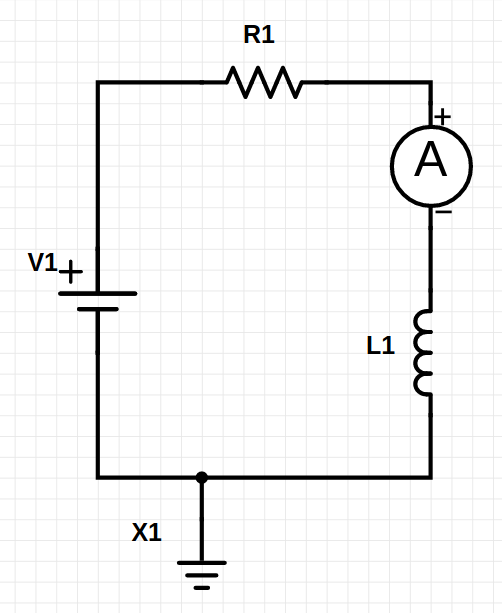
\includegraphics[width=0.3\textwidth]{img/partsim.png}
    \caption{Zapojenie obvodu v Partsim}
\end{figure}

Výpočet rovnicou ($t=\SI{1.5}{\second}$):

\begin{equation*}
\begin{aligned}
i_L(1.5)&=\frac{30}{20}(1-e^{-\frac{20}{10}*1.5})+15e^{-\frac{20}{10}*1.5} \\
i_L(1.5) &\approx \SI{2.172125423}{\ampere}
\end{aligned}
\end{equation*}

\newpage

Výsledok v Partsim:

\begin{figure}[h!]
    \centering
    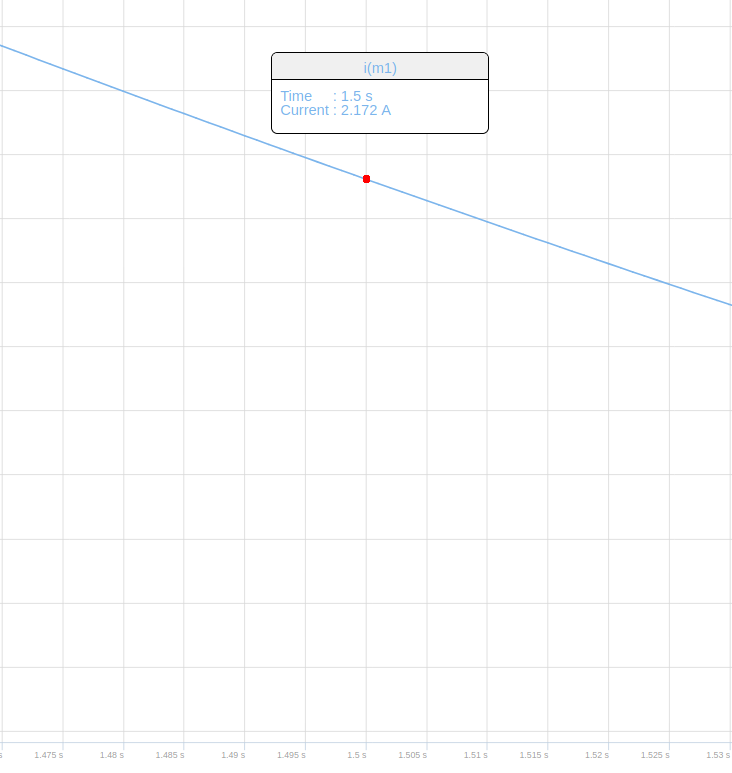
\includegraphics[width=0.8\textwidth]{img/graf.png}
    \caption{$i_L(\SI{1.5}{\second})$}
\end{figure}








    \section{Výsledky}

\begin{tabularx}{\textwidth}{|c|c|X|}
	\hline
	\textbf{Úloha} & \textbf{Skupina} & \textbf{Výsledok} \\
	\hline
	\multirow{2}{*}{\textbf{1}} &A & $U_{R_{6}} \approx \SI{68.929}{\volt}$ \\
	& & $I_{R_{6}} \approx \SI{0.0919}{\ampere}$ \\
	\hline
	\multirow{2}{*}{\textbf{2}} &B & $U_{R_{3}} \approx \SI{42.9586}{\volt}$ \\
	& & $I_{R_{3}} \approx \SI{70.424}{\milli \ampere}$ \\
	\hline
	\multirow{2}{*}{\textbf{3}} &G & $U_{R_{2}} \approx \SI{68.788}{\volt}$ \\
	& & $I_{R_{2}} \approx \SI{1.6778}{\ampere}$ \\
	\hline
	\multirow{2}{*}{\textbf{4}} &A & $|U_{L_{2}}| \approx \SI{10.443}{\volt}$ \\
	& & $\varphi_{L_{2}} \approx \SI{0.459}{\radian}$ \\
	\hline
    \textbf{5} &B & $i_L(t)=e^{-2t} \times \frac{27}{2} + \frac{3}{2}$ \\
	\hline
\end{tabularx}

\end{document}